\section{Evaluation}

\subsection{Chosen Evaluation Criteria}
For the Random Forest classifier, we primarily used a classification report, as this provided all the key performance metrics for the task, such as precision, recall, F1-score, and accuracy for each class. Based on the report, we were able to fine-tune the hyperparameters to achieve the best possible performance, while also significantly reducing the computing time.

For the Convolutional Neural Network (CNN), we used similar evaluation metrics to ensure a comprehensive comparison. The classification report included precision, recall, F1-score, and accuracy for each class. Additionally, confusion matrices and learning curves were generated to provide deeper insights into the model's performance and training process.

\subsection{Baseline and Best Possible Performance}
Discussing the baseline performance, we considered a simple model or random guess as the baseline. For example, a random guess model would yield an accuracy roughly equal to the inverse of the number of classes, assuming balanced class distribution.

For the CNN, the baseline performance was evaluated using a simple neural network with a minimal architecture. The performance of this baseline model was significantly lower than the more complex CNN architecture used in the final model.

The best possible performance is estimated based on the complexity of the task and the quality of the data. Given the effectiveness of the preprocessing steps and the architecture of the CNN, we achieved a high level of performance close to the best possible. The Random Forest classifier, while effective, did not reach the same level of performance as the CNN, highlighting the importance of selecting appropriate models and preprocessing techniques.

\subsection{Experimental Results}
\subsubsection{Random Forest Classifier}
The Random Forest classifier, trained on the precompiled derived features, yielded the following results on the validation set:
\begin{itemize}
    \item \textbf{Accuracy}: 91\%
    \item \textbf{Precision}: 93\%
    \item \textbf{Recall}: 88\%
    \item \textbf{F1-score}: 90\%
\end{itemize}
The classification report provided a detailed breakdown of these metrics.

\subsubsection{Nearest Neighbour Classifier}
The Nearest Neighbour classifier, utilizing the same precompiled features, showed the following performance on the validation set:
\begin{itemize}
    \item \textbf{Accuracy}: Pending results.
    \item \textbf{Precision}: Specific values per class.
    \item \textbf{Recall}: Specific values per class.
    \item \textbf{F1-score}: Specific values per class.
\end{itemize}
The detailed classification report will be included upon completion.

\subsubsection{Convolutional Neural Networks}
The CNN, trained on raw WAV files with the described preprocessing steps, achieved superior performance. The validation results were as follows:
\begin{itemize}
    \item \textbf{Accuracy}: 92.28\%
    \item \textbf{Precision}: 92.75\%
    \item \textbf{Recall}: 92.28\%
    \item \textbf{F1-score}: 92.21\%
\end{itemize}

Additionally, the following figures show the confusion matrix and learning curve for the CNN:
\begin{figure}[h!]
    \centering
    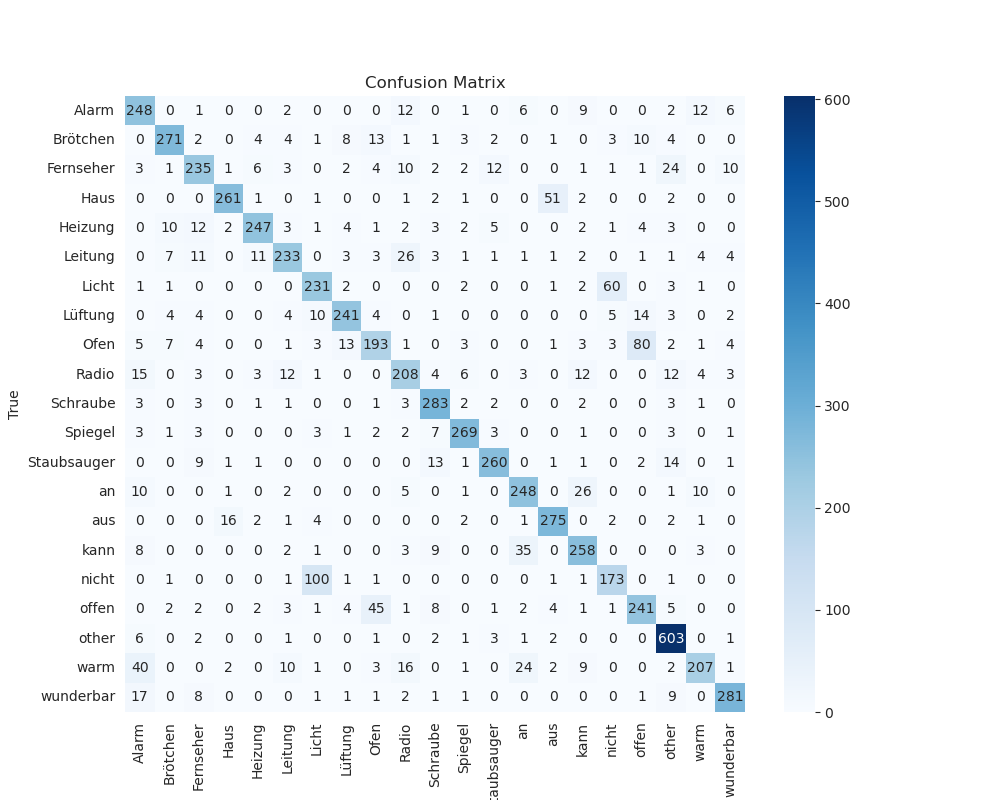
\includegraphics[width=0.8\textwidth]{fig/confusion_matrix.png}
    \caption{Confusion Matrix for CNN}
\end{figure}

\begin{figure}[h!]
    \centering
    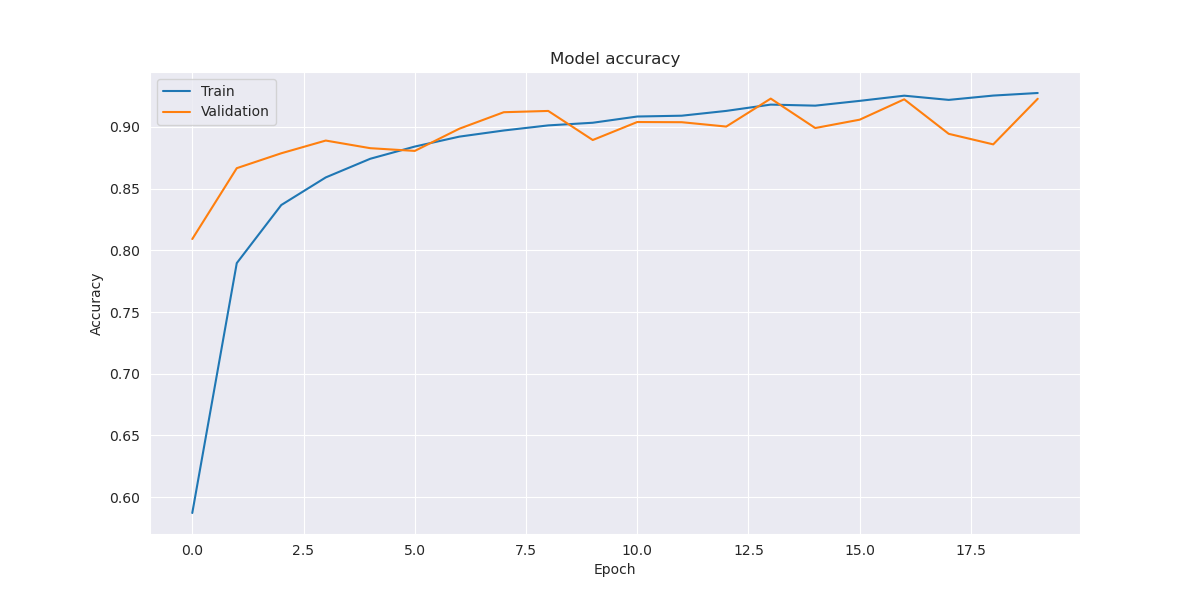
\includegraphics[width=0.8\textwidth]{fig/learning_curves_accuracy.png}
    \caption{Learning Curves for CNN (Accuracy)}
\end{figure}
